%
% Documento: Anexos
%

\begin{anexosenv}
\partanexos

\chapter{Resultados Catálogo selec20}
\label{chap:anexoselec20}

Com a aplicação do nosso método nos 20 aglomerados do catálogo selec20 obtivemos os seguintes resultados, dado o histograma de velocidade, o eixo principal e o perfil de rotação apenas para os aglomerados que apresentaram rotação significativa.  

\begin{figure}[H] %h or !htbp
\vspace{-2pt}
\centering
\subfloat{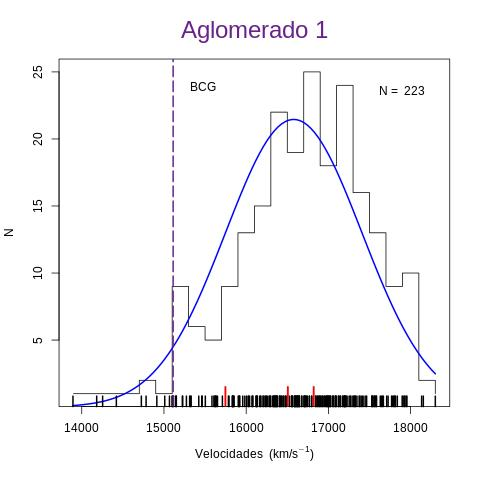
\includegraphics[scale=.23]{04-figuras/selec20/dist01}}
\subfloat{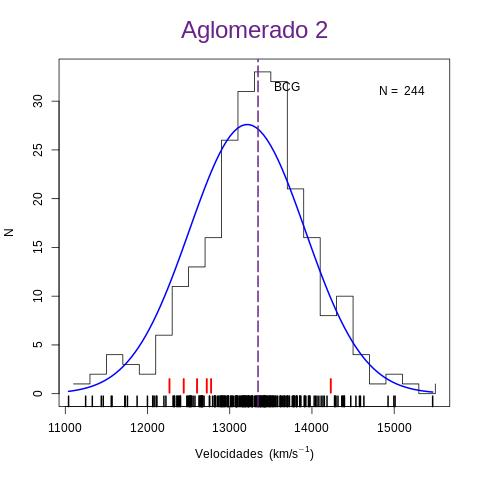
\includegraphics[scale=.23]{04-figuras/selec20/dist02}}
\subfloat{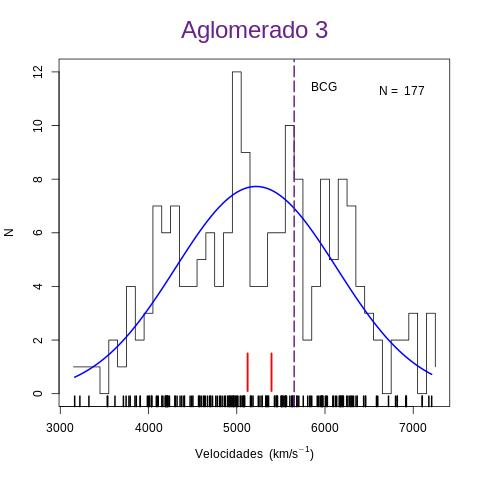
\includegraphics[scale=.23]{04-figuras/selec20/dist03}}
\subfloat{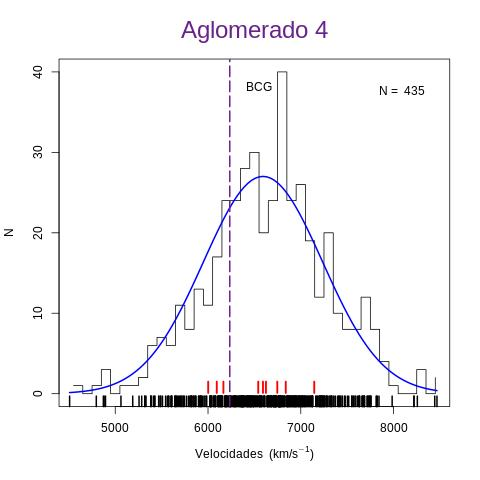
\includegraphics[scale=.23]{04-figuras/selec20/dist04}}\hfill
\subfloat{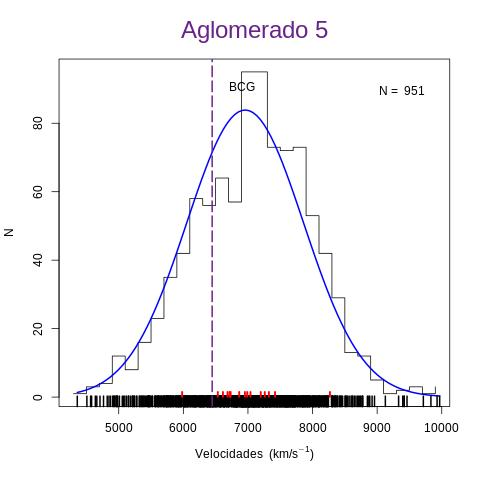
\includegraphics[scale=.23]{04-figuras/selec20/dist05}}
\subfloat{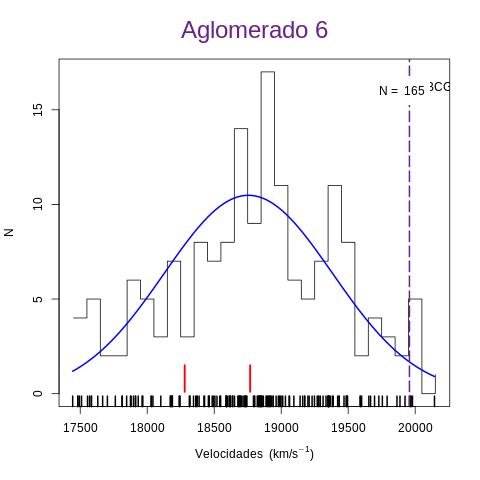
\includegraphics[scale=.23]{04-figuras/selec20/dist06}}
\subfloat{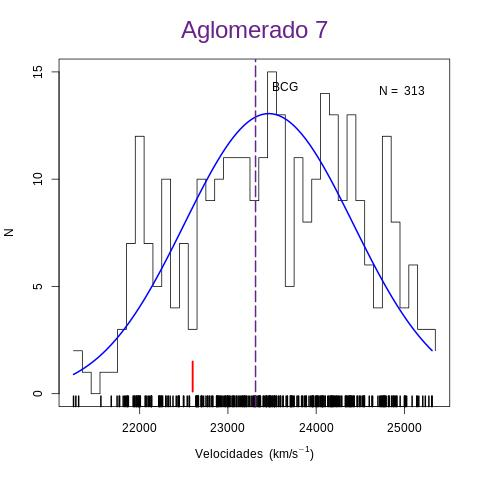
\includegraphics[scale=.23]{04-figuras/selec20/dist07}}
\subfloat{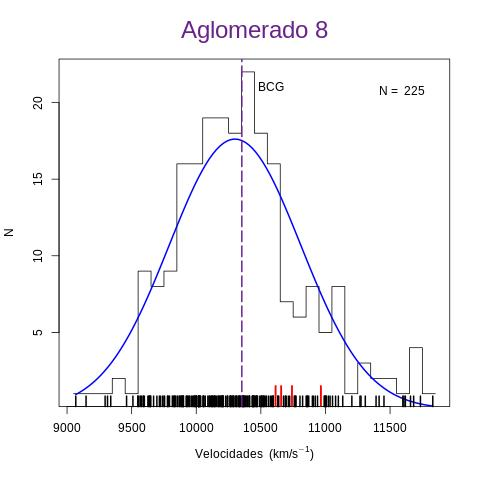
\includegraphics[scale=.23]{04-figuras/selec20/dist08}}\hfill
\subfloat{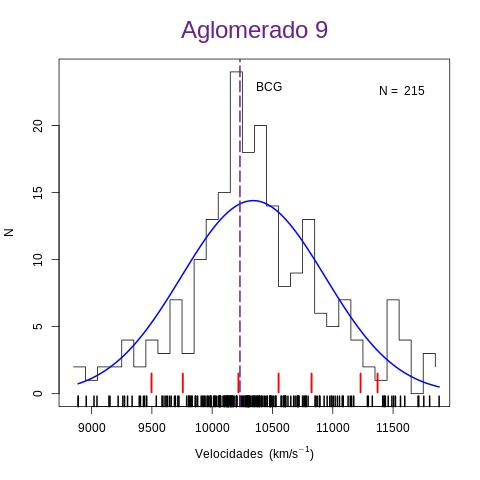
\includegraphics[scale=.23]{04-figuras/selec20/dist09}}
\subfloat{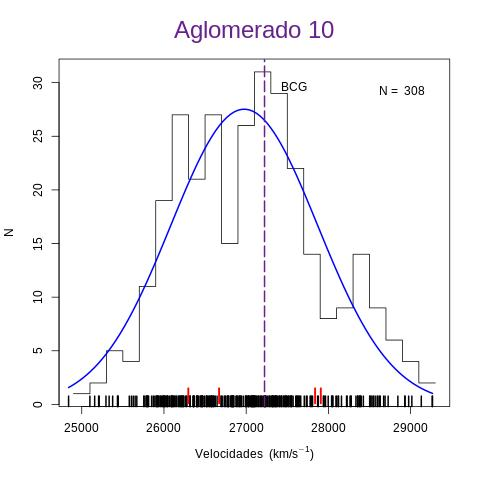
\includegraphics[scale=.23]{04-figuras/selec20/dist10}}
\subfloat{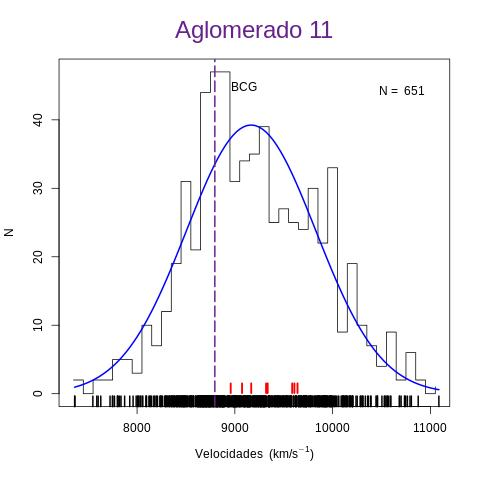
\includegraphics[scale=.23]{04-figuras/selec20/dist11}}
\subfloat{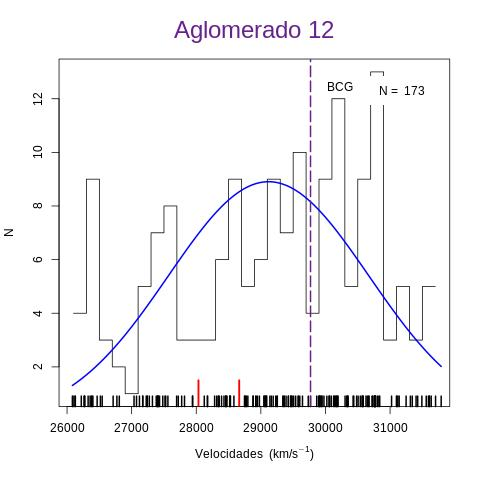
\includegraphics[scale=.23]{04-figuras/selec20/dist12}}\hfill
\subfloat{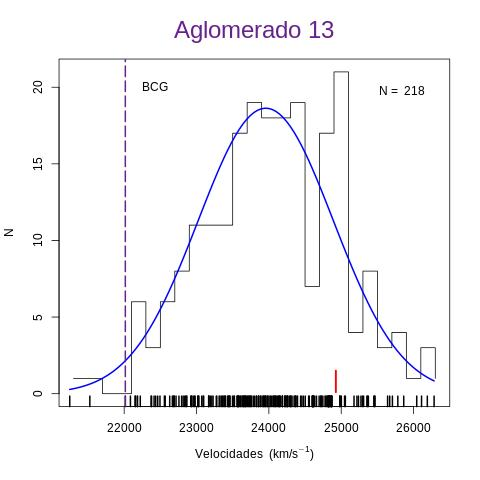
\includegraphics[scale=.23]{04-figuras/selec20/dist13}}
\subfloat{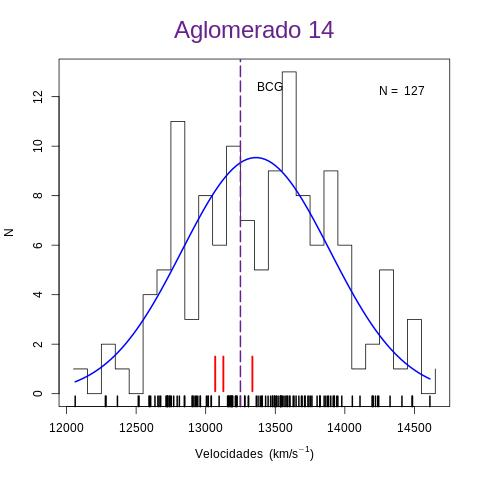
\includegraphics[scale=.23]{04-figuras/selec20/dist14}}
\subfloat{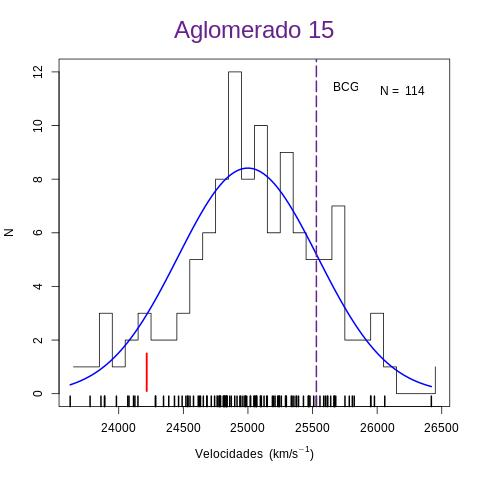
\includegraphics[scale=.23]{04-figuras/selec20/dist15}}
\subfloat{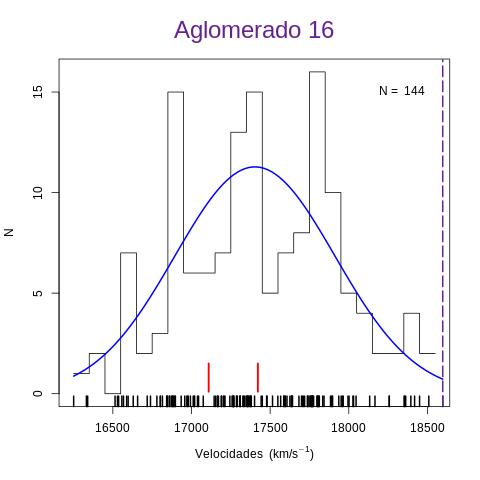
\includegraphics[scale=.23]{04-figuras/selec20/dist16}}\hfill
\subfloat{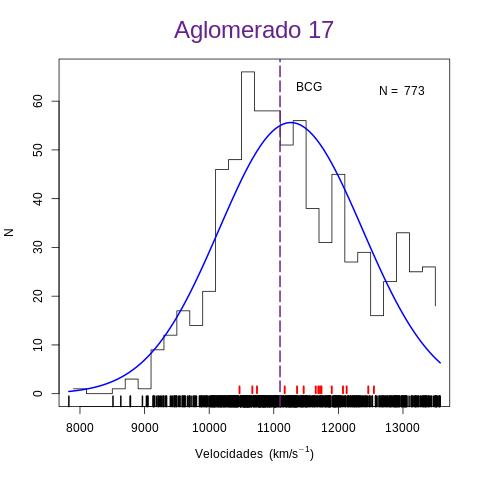
\includegraphics[scale=.23]{04-figuras/selec20/dist17}}
\subfloat{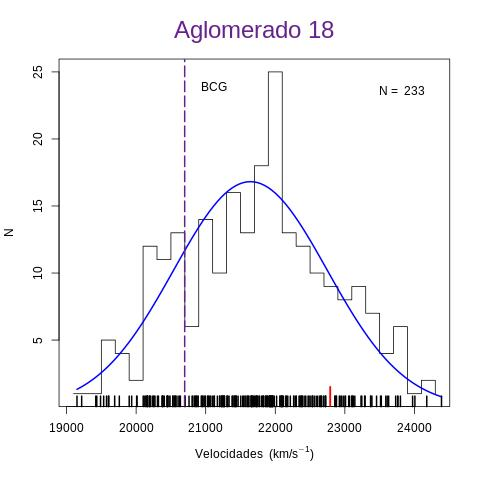
\includegraphics[scale=.23]{04-figuras/selec20/dist18}}
\subfloat{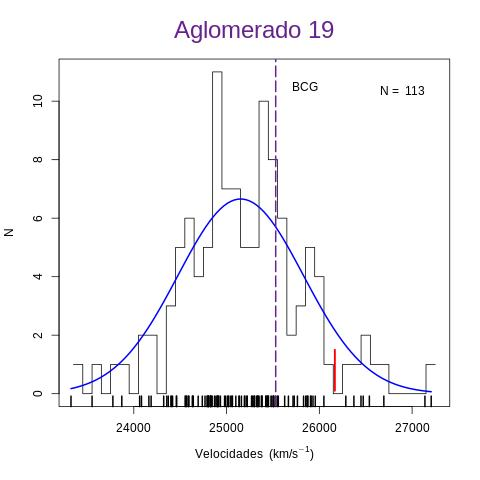
\includegraphics[scale=.23]{04-figuras/selec20/dist19}}
\subfloat{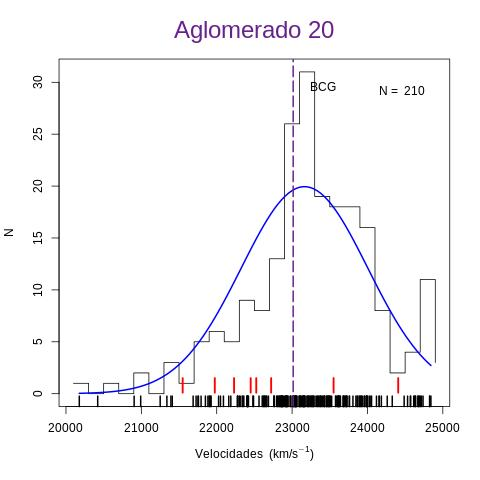
\includegraphics[scale=.23]{04-figuras/selec20/dist20}}
\caption{Histograma Distribuição de Velocidade e Análise de Gaps.}
\label{fig:fig4}%
\end{figure}


\begin{figure}[H] %h or !htbp
\vspace{-2pt}
\begin{center}
\subfloat{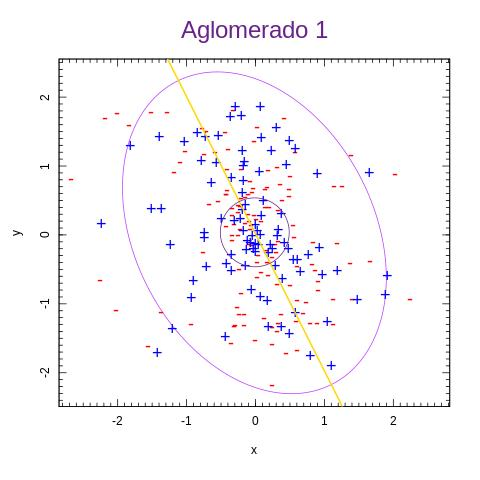
\includegraphics[scale=.23]{04-figuras/selec20/eixo01}}
\subfloat{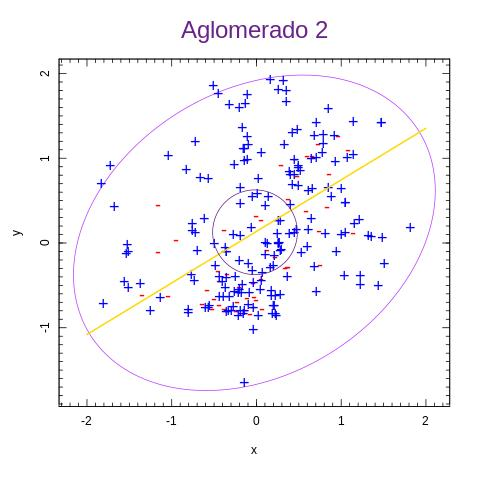
\includegraphics[scale=.23]{04-figuras/selec20/eixo02}}
\subfloat{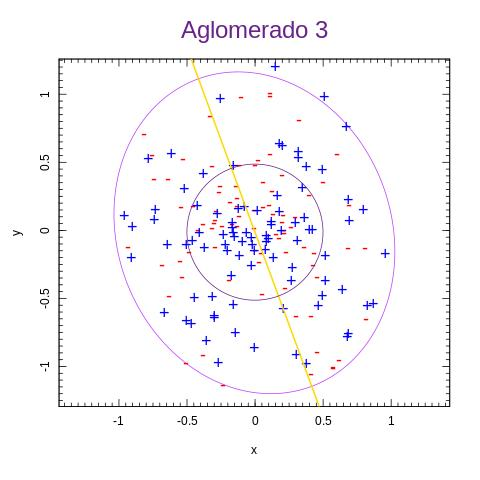
\includegraphics[scale=.23]{04-figuras/selec20/eixo03}}
\subfloat{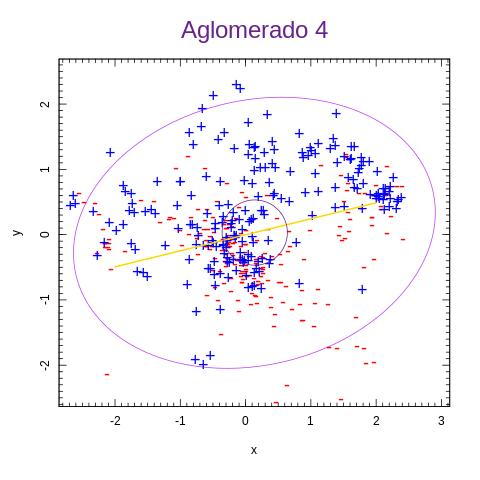
\includegraphics[scale=.23]{04-figuras/selec20/eixo04}}\hfill
\subfloat{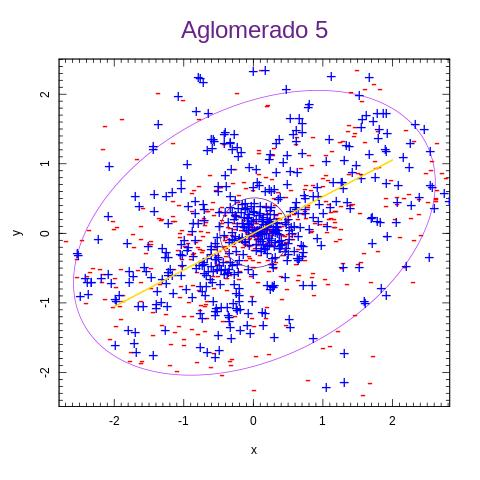
\includegraphics[scale=.23 ]{04-figuras/selec20/eixo05}}
\subfloat{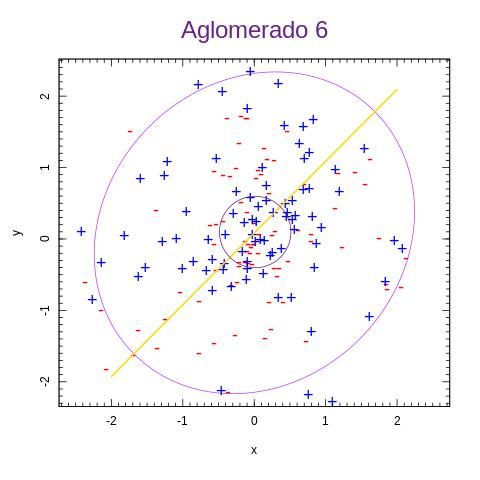
\includegraphics[scale=.23 ]{04-figuras/selec20/eixo06}}
\subfloat{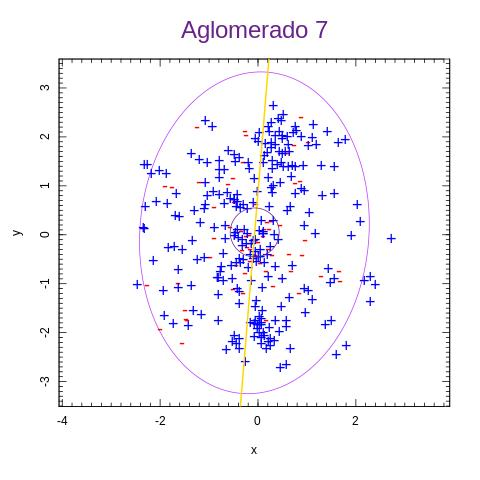
\includegraphics[scale=.23 ]{04-figuras/selec20/eixo07}}
\subfloat{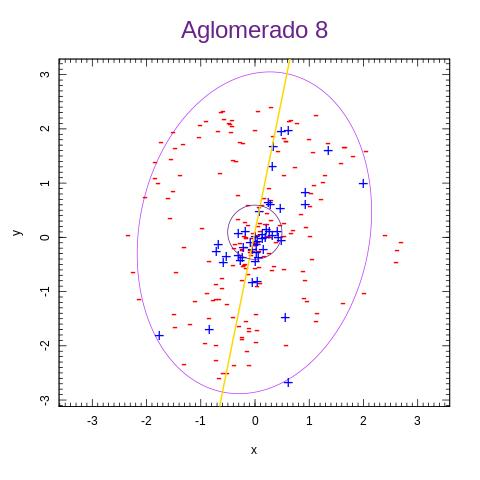
\includegraphics[scale=.23 ]{04-figuras/selec20/eixo08}}\hfill
\subfloat{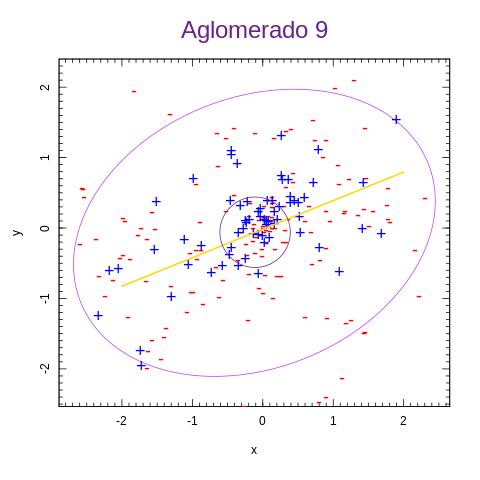
\includegraphics[scale=.23 ]{04-figuras/selec20/eixo09}}
\subfloat{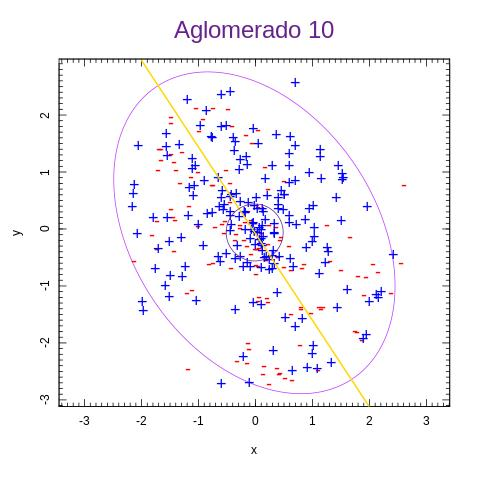
\includegraphics[scale=.23 ]{04-figuras/selec20/eixo10}}
\subfloat{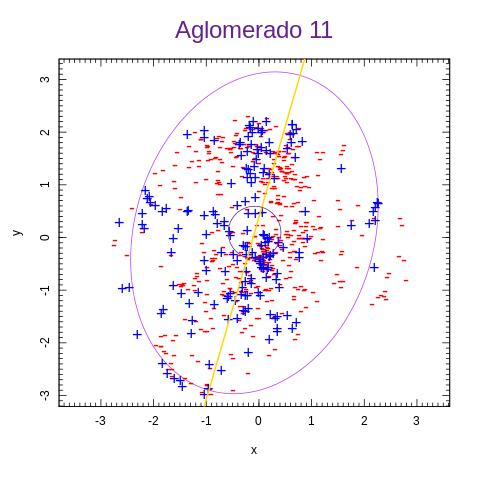
\includegraphics[scale=.23 ]{04-figuras/selec20/eixo11}}
\subfloat{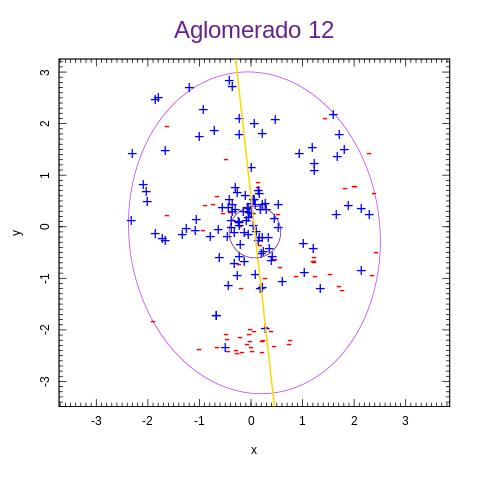
\includegraphics[scale=.23 ]{04-figuras/selec20/eixo12}}\hfill
\subfloat{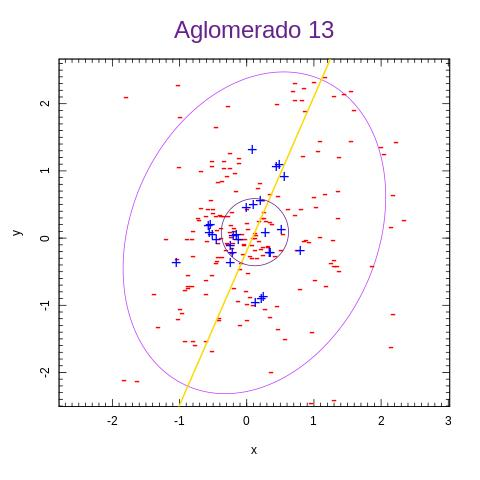
\includegraphics[scale=.23 ]{04-figuras/selec20/eixo13}}
\subfloat{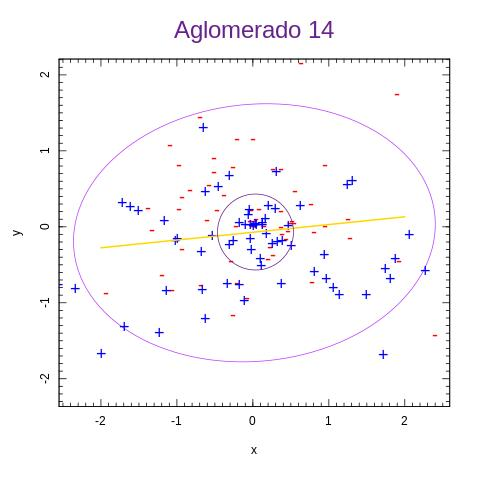
\includegraphics[scale=.23 ]{04-figuras/selec20/eixo14}}
\subfloat{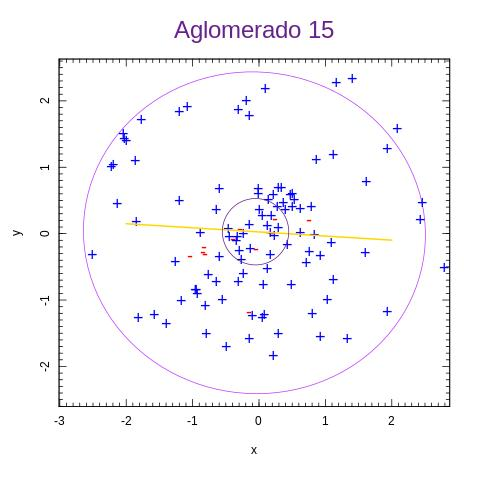
\includegraphics[scale=.23 ]{04-figuras/selec20/eixo15}}
\subfloat{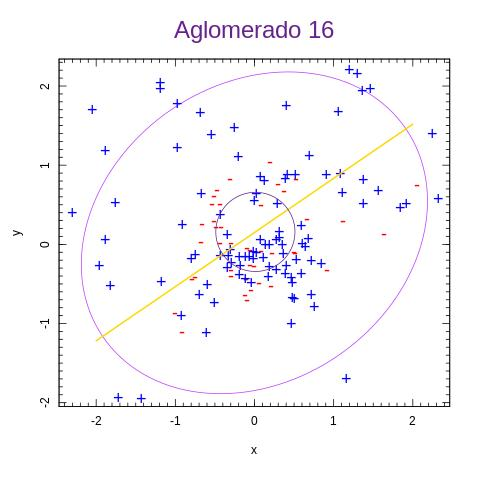
\includegraphics[scale=.23 ]{04-figuras/selec20/eixo16}}\hfill
\subfloat{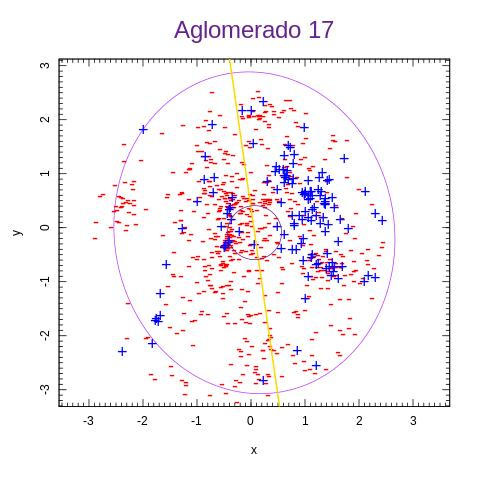
\includegraphics[scale=.23 ]{04-figuras/selec20/eixo17}}
\subfloat{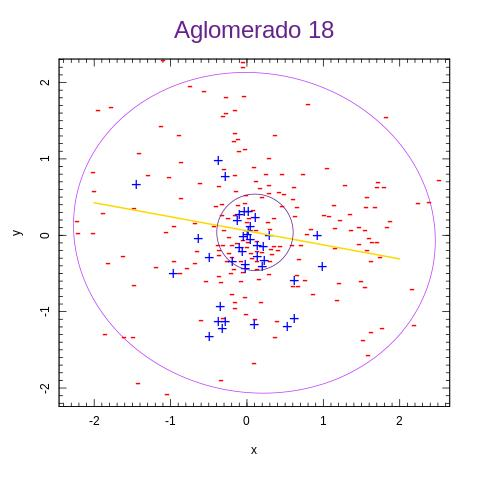
\includegraphics[scale=.23 ]{04-figuras/selec20/eixo18}}
\subfloat{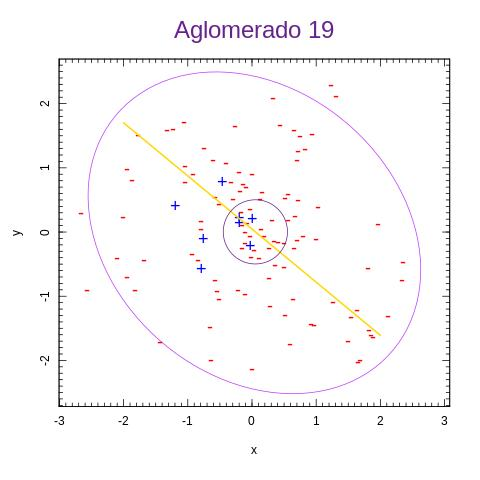
\includegraphics[scale=.23 ]{04-figuras/selec20/eixo19}}
\subfloat{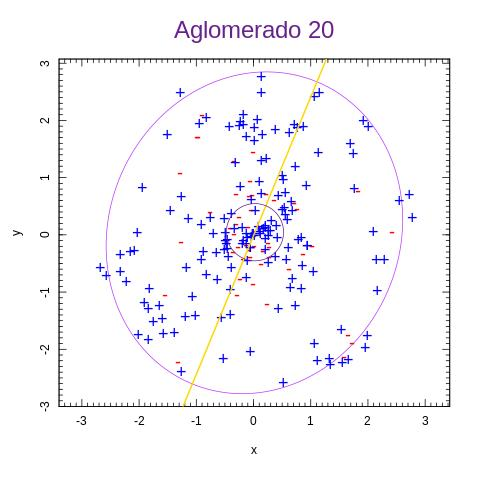
\includegraphics[scale=.23 ]{04-figuras/selec20/eixo20}}
\caption{Ajuste da elipse e eixo principal da distribuição projetada no plano do céu.}
\label{fig5}%
\end{center}
\end{figure}


\begin{figure}[H] %h or !htbp
\vspace{-2pt}
\begin{center}
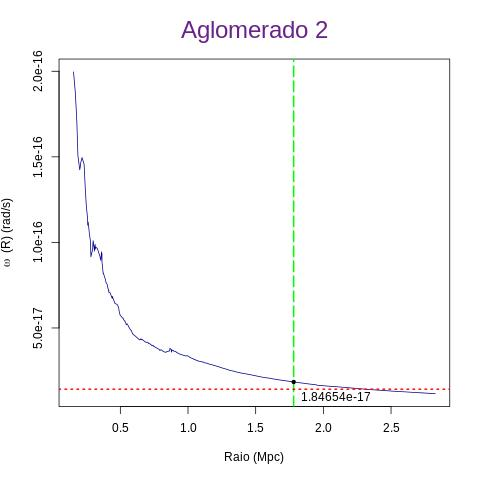
\includegraphics[scale=.3]{04-figuras/selec20/perfil02}%
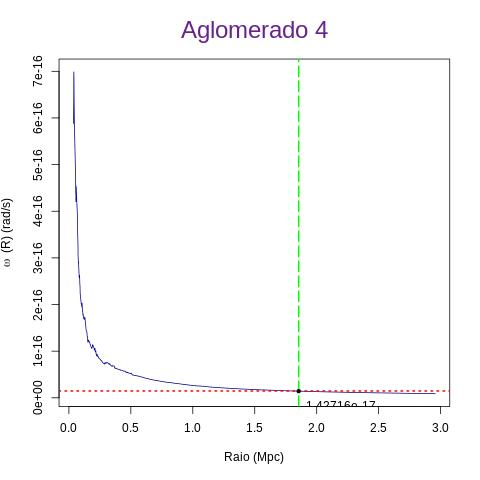
\includegraphics[scale=.3]{04-figuras/selec20/perfil04}
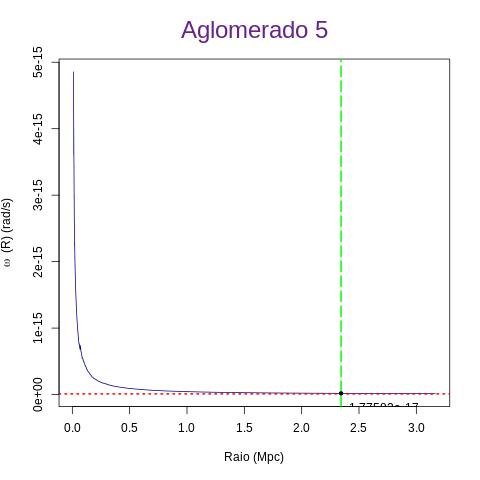
\includegraphics[scale=.3]{04-figuras/selec20/perfil05}
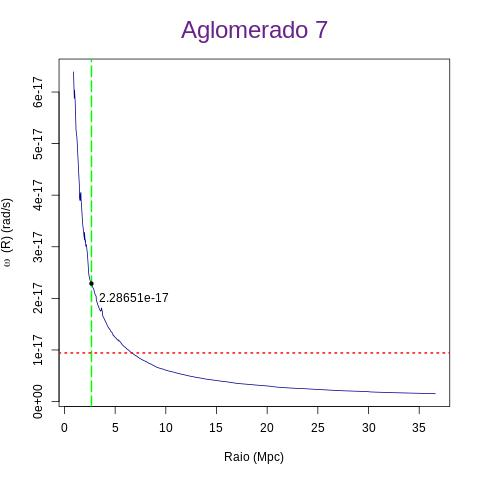
\includegraphics[scale=.3]{04-figuras/selec20/perfil07}\hfill
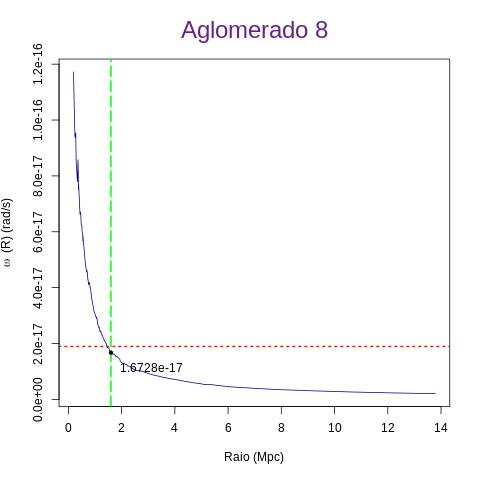
\includegraphics[scale=.3]{04-figuras/selec20/perfil08}
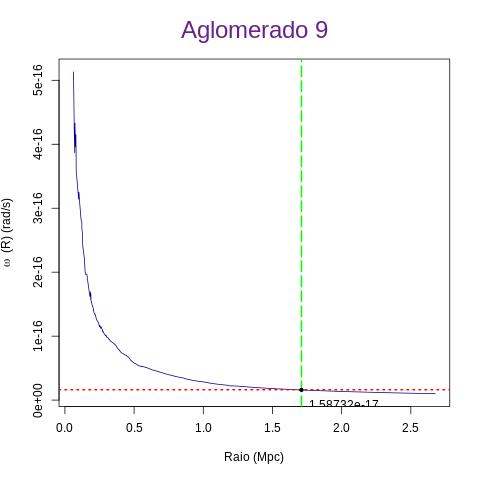
\includegraphics[scale=.3]{04-figuras/selec20/perfil09}
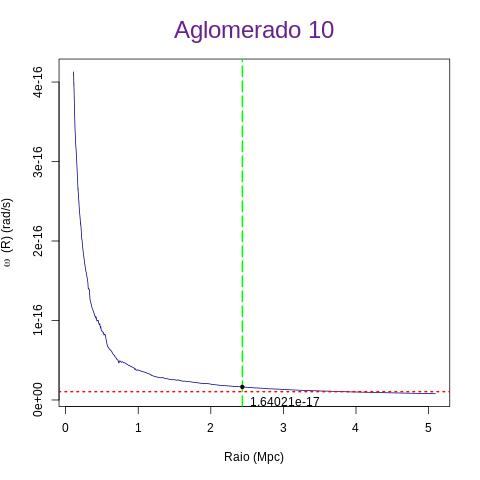
\includegraphics[scale=.3]{04-figuras/selec20/perfil10}
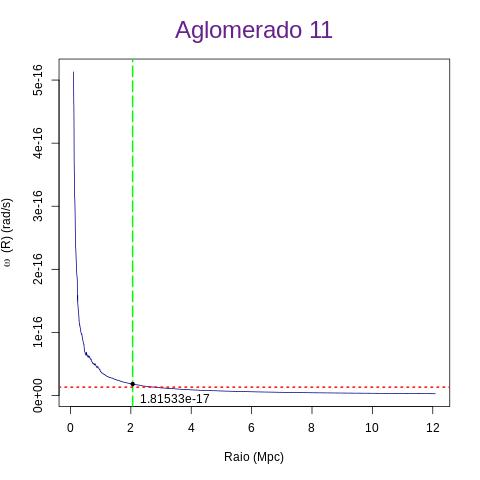
\includegraphics[scale=.3]{04-figuras/selec20/perfil11}\hfill
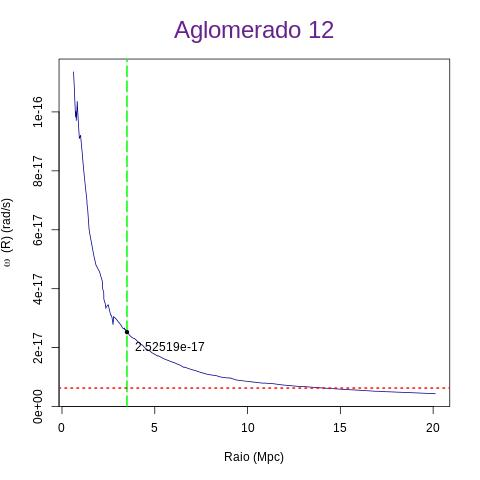
\includegraphics[scale=.3]{04-figuras/selec20/perfil12}
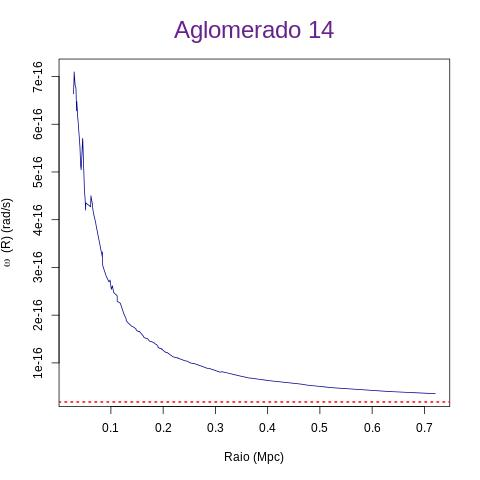
\includegraphics[scale=.3]{04-figuras/selec20/perfil14}
\includegraphics[scale=.3]{04-figuras/selec20/perfil15}
\includegraphics[scale=.3]{04-figuras/selec20/perfil16}\hfill
\includegraphics[scale=.3]{04-figuras/selec20/perfil17}
\includegraphics[scale=.3]{04-figuras/selec20/perfil18}
\caption{Perfil da velocidade de rotação.}
\label{fig6}%
\end{center}
\end{figure}

\chapter{Resultados Catálogo NoSOCS}
\label{chap:anexonosocs}
Os resultados obtidos na aplicação do nosso método para o catálogo NoSOCS são os seguintes, dado o histograma de velocidade, o eixo principal, a tabela comparativa dos testes utilizados (Cramer e Hotelling) e o perfil de rotação apenas para os aglomerados que apresentaram rotação significativa.

\begin{table}[H]
\caption{Teste Cramer e Hotelling aplicado no catálogo NoSOCS utilizando gap - sem indicação rotação.}
\vspace{12pt}
\centering{}
\resizebox{.8\textwidth}{!}{
\begin{tabular}{|l|l|l|l|l|l|l|l|}
\hline
\multirow{2}{*}{\textbf{Cluster}} & \multicolumn{2}{c|}{\textbf{Cenário 1}} & \multicolumn{2}{c|}{\textbf{Cenário 2}} & \multicolumn{2}{c|}{\textbf{Cenário 3}} & \multirow{2}{*}{\textbf{Nº galáxias}} \\ \cline{2-7}
                         & \textbf{Cramer}       & \textbf{Hotelling}       & \textbf{Cramer}       & \textbf{Hotelling}       & \textbf{Cramer}       & \textbf{Hotelling}       &                              \\ \hline
                        00996 & 0.7412587 & 0.8761337 & 0.5254745 & 0.6375903 & 0.4935065 & 0.8687519 & 118 \\ \hline
						01052 & 0.6333666 & 0.9305163 & 0.1148851 & 0.05342577 & 0.2847153 & 0.5574755 & 34 \\ \hline
						01264 & 0.1038961 & 0.1679695 & 0.2257742 & 0.4912261 & NA & NA & 31 \\ \hline
						01347 & 0.4925075 & 0.3881943 & 0.4985015 & 0.6860376 & 0.5344655 & 0.4913995 & 37 \\ \hline
						01933 & 0.3146853 & 0.2462812 & 0.7542458 & 0.7689922 & 0.2857143 & 0.4333554 & 78 \\ \hline
						02301 & 0.0989011 & 0.3656919 & 0.4085914 & 0.6013579 & 0.08791209 & 0.495044 & 75 \\ \hline
						02899 & 0.3666334 & 0.4510812 & 0.3946054 & 0.4849135 & 0.2547453 & 0.5869276 & 44 \\ \hline
						03459 & 0.8231768 & 0.6045021 & 0.4615385 & 0.290978 & 0.963037 & 0.8782925 & 129 \\ \hline
						04404 & 0.5824176 & 0.8435559 & 0.5164835 & 0.8678394 & 0.5784216 & 0.4055207 & 34 \\ \hline
						04405 & 0.2657343 & 0.3529274 & 0.2897103 & 0.36971 & 0.8181818 & 0.942962 & 35 \\ \hline
						04458 & 0.09190809 & 0.2165505 & 0.1958042 & 0.1484606 & 0.1368631 & 0.2482086 & 75 \\ \hline
						05535 & 0.7182817 & 0.4094059 & 0.4365634 & 0.5584254 & 0.2587413 & 0.1105721 & 49 \\ \hline
						05717 & 0.1798202 & 0.5592738 & 0.4015984 & 0.7776702 & 0.3526474 & 0.7187614 & 68 \\ \hline
						05859 & 0.2207792 & 0.1678599 & 0.7592408 & 0.9945818 & 0.7602398 & 0.9039455 & 44 \\ \hline
						05908 & 0.7312687 & 0.6639244 & 0.4885115 & 0.9556211 & 0.6673327 & 0.8438158 & 32 \\ \hline
						06070 & 0.06693307 & 0.6518467 & 0.1618382 & 0.05954166 & 0.1928072 & 0.1794072 & 43 \\ \hline
						06723 & 0.5814186 & 0.7952297 & 0.4435564 & 0.474908 & 0.7402597 & 0.6023129 & 22 \\ \hline
						07837 & 0.2017982 & 0.2020218 & 0.2117882 & 0.08223968 & 0.2937063 & NA & 22 \\ \hline
						07975 & 0.08991009 & 0.05746997 & 0.06793207 & 0.06994625 & 0.4175824 & 0.4909229 & 36 \\ \hline
						08291 & 0.2207792 & 0.2387312 & 0.2027972 & 0.2041885 & 0.5094905 & 0.5338773 & 43 \\ \hline
						08738 & 0.1178821 & 0.4439133 & 0.3286713 & 0.4319458 & 0.2907093 & 0.2139703 & 51 \\ \hline
						08742 & 0.1798202 & 0.8047111 & 0.1018981 & 0.1251147 & 0.3526474 & 0.4534198 & 64 \\ \hline
						09153 & 0.6443556 & 0.7399757 & 0.4125874 & 0.4849873 & 0.2647353 & 0.2816225 & 24 \\ \hline
						10001 & 0.7002997 & 0.5486396 & 0.5944056 & 0.334425 & 0.6723277 & 0.6086176 & 205 \\ \hline
						10004 & 0.06293706 & 0.5419472 & 0.1388611 & 0.433163 & 0.08591409 & 0.1359992 & 86 \\ \hline
						10009 & 0.2237762 & 0.5741624 & 0.4675325 & 0.4290245 & 0.5614386 & 0.8211343 & 62 \\ \hline
						10010 & 0.3386613 & 0.8987447 & 0.4155844 & 0.484555 & 0.6523477 & 0.49937 & 135 \\ \hline
						10014 & 0.6173826 & 0.9580584 & 0.7252747 & 0.6412154 & 0.5714286 & 0.936806 & 39 \\ \hline
						10017 & 0.3016983 & 0.7229228 & 0.07892108 & 0.1712904 & 0.06593407 & 0.4018374 & 88 \\ \hline
						10019 & 0.2897103 & 0.4306538 & 0.1128871 & 0.1846356 & 0.8461538 & 0.8852156 & 142 \\ \hline
						10025 & 0.1358641 & 0.516039 & 0.3946054 & 0.8024935 & 0.1108891 & 0.2339634 & 126 \\ \hline
						10032 & 0.05494505 & 0.2733059 & 0.5364635 & 0.3797048 & 0.1508492 & 0.3255304 & 93 \\ \hline
						10038 & 0.1058941 & 0.5774182 & 0.1648352 & 0.412123 & 0.2837163 & 0.2596397 & 170 \\ \hline
						10041 & 0.4195804 & 0.5239049 & 0.4405594 & 0.7856695 & 0.8511489 & 0.7160758 & 113 \\ \hline
						10042 & 0.3886114 & 0.7649132 & 0.7422577 & 0.6799726 & 0.2027972 & 0.2416632 & 32 \\ \hline
						10048 & 0.5994006 & 0.9850915 & 0.4345654 & 0.7785383 & 0.6643357 & 0.7787913 & 270 \\ \hline
						10058 & 0.3416583 & 0.8175262 & 0.1908092 & 0.08933787 & 0.5124875 & 0.6402473 & 194 \\ \hline
                   
\label{tab:nosocssemrotacaoI}
\end{tabular}
}
\end{table}

\begin{table}[H]
\caption{Teste Cramer e Hotelling aplicado no catálogo NoSOCS utilizando mediana - sem indicação rotação.}
\vspace{12pt}
\centering{}
\resizebox{.8\textwidth}{!}{
\begin{tabular}{|l|l|l|l|l|l|l|l|}
\hline
\multirow{2}{*}{\textbf{Cluster}} & \multicolumn{2}{c|}{\textbf{Cenário 1}} & \multicolumn{2}{c|}{\textbf{Cenário 2}} & \multicolumn{2}{c|}{\textbf{Cenário 3}} & \multirow{2}{*}{\textbf{Nº galáxias}} \\ \cline{2-7}
                         & \textbf{Cramer}       & \textbf{Hotelling}       & \textbf{Cramer}       & \textbf{Hotelling}       & \textbf{Cramer}       & \textbf{Hotelling}       &                              \\ \hline
                        00339 & 0.3316683 & 0.9613848 & 0.2927073 & 0.591892 & 0.8291708 & 0.8731429 & 66 \\ \hline
						01189 & 0.4375624 & 0.4349387 & 0.4675325 & 0.493412 & 0.07492507 & 0.08958739 & 40 \\ \hline
						01877 & 0.2207792 & 0.5432613 & 0.4055944 & 0.2932482 & 0.3836164 & 0.7414256 & 28 \\ \hline
						02104 & 0.1458541 & 0.2732179 & 0.2337662 & 0.1225379 & 0.6023976 & 0.5387223 & 48 \\ \hline
						02298 & 0.3016983 & 0.6269575 & 0.2077922 & 0.1750384 & 0.6743257 & 0.6889499 & 29 \\ \hline
						02469 & 0.3956044 & 0.6919376 & 0.08091908 & NA & 0.06393606 & 0.1412525 & 26 \\ \hline
						02490 & 0.6793207 & NA & 0.3896104 & NA & - & - & 24 \\ \hline
						02752 & 0.4945055 & 0.594916 & 0.498002 & 0.7631145 & 0.5644356 & 0.6835324 & 27 \\ \hline
						03112 & 0.6373626 & 0.9296171 & 0.3806194 & 0.5115455 & 0.4135864 & 0.5982676 & 27 \\ \hline
						03229 & 0.1968032 & 0.3636636 & 0.6583417 & NA & 0.5834166 & 0.9801198 & 36 \\ \hline
						03565 & 0.2417582 & 0.09731901 & 0.3676324 & 0.07157691 & 0.5794206 & 0.3825159 & 33 \\ \hline
						03742 & 0.8811189 & 0.864134 & 0.2367632 & 0.3934403 & 0.4575425 & 0.5633551 & 74 \\ \hline
						03898 & 0.2317682 & 0.4892585 & 0.1458541 & 0.5520248 & 0.3776224 & 0.4105107 & 30 \\ \hline
						03915 & 0.08191808 & 0.3495027 & 0.3526474 & 0.4467789 & 0.05394605 & 0.05046389 & 67 \\ \hline
						03975 & 0.2087912 & 0.1740886 & 0.5484515 & 0.6921665 & 0.5404595 & 0.5736747 & 33 \\ \hline
						04023 & 0.2637363 & 0.4502279 & 0.7682318 & 0.8864958 & 0.1548452 & 0.1767911 & 93 \\ \hline
						04100 & 0.3676324 & 0.2932311 & 0.6093906 & 0.8529075 & 0.1608392 & 0.1241679 & 37 \\ \hline
						04376 & 0.2637363 & 0.3737319 & 0.2627373 & 0.1573387 & 0.2397602 & 0.1663829 & 29 \\ \hline
						04710 & 0.7262737 & NA & - & - & 0.6823177 & NA & 29 \\ \hline
						05039 & 0.2937063 & 0.2833302 & 0.3266733 & 0.5049447 & 0.7352647 & NA & 29 \\ \hline
						05206 & 0.6853147 & 0.7371136 & 0.3256743 & 0.4527116 & 0.7012987 & 0.9924852 & 26 \\ \hline
						05325 & 0.3116883 & 0.5188909 & 0.05894106 & 0.1093263 & 0.8211788 & 0.9761832 & 24 \\ \hline
						06173 & 0.3286713 & 0.3997239 & 0.2887113 & 0.5266079 & 0.3086913 & 0.211082 & 62 \\ \hline
						06175 & 0.07392607 & 0.09310988 & 0.3316683 & 0.4934143 & 0.2217782 & NA & 21 \\ \hline
						06184 & 0.3386613 & 0.9743288 & 0.3656344 & 0.6413506 & 0.3746254 & 0.6746557 & 28 \\ \hline
						06233 & 0.2697303 & 0.1376332 & 0.1178821 & 0.182314 & 0.1738262 & 0.2156128 & 42 \\ \hline
						06261 & 0.4545455 & 0.5955426 & 0.969031 & 0.9682067 & 0.07192807 & 0.1983339 & 48 \\ \hline
						06264 & 0.4865135 & 0.8170953 & 0.2637363 & 0.2610734 & 0.1328671 & 0.3385866 & 24 \\ \hline
						06392 & 0.2587413 & 0.2429681 & 0.1578422 & 0.2800286 & 0.5954046 & 0.7202507 & 46 \\ \hline
						06447 & 0.2157842 & 0.2377592 & 0.2337662 & 0.3918406 & 0.2897103 & 0.4684874 & 48 \\ \hline
						06475 & 0.3516484 & 0.3046087 & 0.2087912 & 0.4157828 & 0.3726274 & 0.2559057 & 52 \\ \hline
						06506 & 0.3516484 & 0.9908666 & 0.08191808 & 0.2413385 & 0.1388611 & 0.3520774 & 50 \\ \hline
						06508 & 0.4075924 & 0.291536 & 0.6413586 & 0.6564704 & 0.4395604 & 0.5430494 & 26 \\ \hline
						06841 & 0.1098901 & 0.09076928 & 0.5114885 & 0.4045139 & 0.1728272 & 0.4598884 & 40 \\ \hline
						06924 & 0.2897103 & 0.3820041 & 0.7862138 & NA & 0.3956044 & 0.4781404 & 27 \\ \hline
						07204 & 0.5314685 & 0.9523549 & - & - & 0.4445554 & 0.3492997 & 23 \\ \hline
						07435 & 0.5204795 & 0.4180746 & 0.5534466 & 0.8188478 & 0.6543457 & 0.8206986 & 42 \\ \hline
						07520 & 0.1968032 & 0.08573181 & 0.2387612 & 0.2867437 & 0.3396603 & 0.4175084 & 37 \\ \hline
						07775 & 0.2177822 & 0.3310387 & 0.6363636 & 0.8227961 & 0.1688312 & 0.2417417 & 28 \\ \hline
						08173 & 0.4305694 & 0.4044097 & 0.2467532 & 0.335351 & 0.1478521 & NA & 24 \\ \hline
						08219 & 0.1438561 & 0.2354117 & 0.1748252 & 0.28046 & 0.1028971 & 0.1630291 & 26 \\ \hline
						08710 & 0.6413586 & 0.4951129 & 0.6943057 & 0.7955202 & 0.3746254 & 0.2338959 & 48 \\ \hline
						08720 & 0.6603397 & 0.9053504 & 0.1968032 & 0.6057862 & 0.3106893 & 0.4077685 & 27 \\ \hline
						08975 & 0.1158841 & 0.2638592 & 0.4695305 & 0.537334 & 0.06693307 & 0.08576067 & 47 \\ \hline
						09132 & 0.7582418 & 0.9657321 & 0.6493506 & 0.6231385 & 0.3536464 & 0.9450608 & 24 \\ \hline
						09157 & 0.6443556 & 0.9126247 & 0.6483516 & 0.7453382 & 0.5104895 & 0.5389693 & 43 \\ \hline
						09162 & 0.1798202 & 0.3738092 & 0.3826174 & 0.5206843 & 0.3536464 & 0.4131878 & 60 \\ \hline
						09176 & 0.1068931 & 0.4251618 & 0.2897103 & 0.3069839 & 0.08391608 & 0.9942048 & 97 \\ \hline
						09177 & 0.7992008 & 0.7533358 & 0.6313686 & 0.3442569 & 0.7092907 & 0.9310269 & 67 \\ \hline
						10022 & 0.08691309 & 0.1801369 & 0.4775225 & 0.9737396 & 0.1028971 & 0.1139537 & 83 \\ \hline
						10033 & 0.06293706 & 0.1825491 & 0.2547453 & 0.4373272 & 0.3606394 & 0.5479943 & 88 \\ \hline
						10034 & 0.2257742 & 0.1639371 & 0.6453546 & 0.5191255 & 0.1278721 & 0.1358507 & 62 \\ \hline
						10039 & 0.1828172 & 0.7297942 & - & - & 0.1838162 & 0.3686319 & 85 \\ \hline
						10046 & 0.4685315 & 0.1671496 & 0.5834166 & 0.3850925 & 0.8341658 & 0.6650416 & 53 \\ \hline
						10047 & 0.2937063 & 0.5173704 & 0.7602398 & 0.3851868 & 0.0959041 & 0.1480843 & 114 \\ \hline
						10049 & 0.09390609 & 0.07760296 & 0.7232767 & 0.4297825 & 0.3326673 & 0.5222666 & 69 \\ \hline
						10052 & 0.2527473 & 0.5931432 & 0.6613387 & 0.8109619 & 0.2927073 & 0.1249226 & 66 \\ \hline
						10062 & 0.8101898 & 0.5488856 & 0.6333666 & 0.4049079 & 0.1678322 & 0.1822241 & 50 \\ \hline      
\label{tab:nosocssemrotacaoII}
\end{tabular}
}
\end{table}

\begin{figure}[H] %h or !htbp
\vspace{-2pt}
\centering
\subfloat{\includegraphics[scale=.23]{04-figuras/nosocs/dist00339}}
\subfloat{\includegraphics[scale=.23]{04-figuras/nosocs/dist00996}}
\subfloat{\includegraphics[scale=.23]{04-figuras/nosocs/dist01052}}
\subfloat{\includegraphics[scale=.23]{04-figuras/nosocs/dist01189}}\hfill
\subfloat{\includegraphics[scale=.23]{04-figuras/nosocs/dist01238}}
\subfloat{\includegraphics[scale=.23]{04-figuras/nosocs/dist01264}}
\subfloat{\includegraphics[scale=.23]{04-figuras/nosocs/dist01347}}
\subfloat{\includegraphics[scale=.23]{04-figuras/nosocs/dist01831}}\hfill
\subfloat{\includegraphics[scale=.23]{04-figuras/nosocs/dist01836}}
\subfloat{\includegraphics[scale=.23]{04-figuras/nosocs/dist01877}}
\subfloat{\includegraphics[scale=.23]{04-figuras/nosocs/dist01933}}
\subfloat{\includegraphics[scale=.23]{04-figuras/nosocs/dist02104}}\hfill
\subfloat{\includegraphics[scale=.23]{04-figuras/nosocs/dist02137}}
\subfloat{\includegraphics[scale=.23]{04-figuras/nosocs/dist02298}}
\subfloat{\includegraphics[scale=.23]{04-figuras/nosocs/dist02301}}
\subfloat{\includegraphics[scale=.23]{04-figuras/nosocs/dist02433}}\hfill
\subfloat{\includegraphics[scale=.23]{04-figuras/nosocs/dist02440}}
\subfloat{\includegraphics[scale=.23]{04-figuras/nosocs/dist02447}}
\subfloat{\includegraphics[scale=.23]{04-figuras/nosocs/dist02469}}
\subfloat{\includegraphics[scale=.23]{04-figuras/nosocs/dist02490}}\hfill
\subfloat{\includegraphics[scale=.23]{04-figuras/nosocs/dist02752}}
\subfloat{\includegraphics[scale=.23]{04-figuras/nosocs/dist02899}}
\subfloat{\includegraphics[scale=.23]{04-figuras/nosocs/dist03112}}
\subfloat{\includegraphics[scale=.23]{04-figuras/nosocs/dist03176}}
\caption{Histograma Distribuição de Velocidade e Análise de Gaps.}
\label{fig:fig4}%
\end{figure}

\begin{figure}[H] %h or !htbp
\vspace{-2pt}
\centering
\subfloat{\includegraphics[scale=.23]{04-figuras/nosocs/dist03229}}
\subfloat{\includegraphics[scale=.23]{04-figuras/nosocs/dist03459}}
\subfloat{\includegraphics[scale=.23]{04-figuras/nosocs/dist03565}}
\subfloat{\includegraphics[scale=.23]{04-figuras/nosocs/dist03691}}\hfill
\subfloat{\includegraphics[scale=.23]{04-figuras/nosocs/dist03742}}
\subfloat{\includegraphics[scale=.23]{04-figuras/nosocs/dist03898}}
\subfloat{\includegraphics[scale=.23]{04-figuras/nosocs/dist03907}}
\subfloat{\includegraphics[scale=.23]{04-figuras/nosocs/dist03915}}\hfill
\subfloat{\includegraphics[scale=.23]{04-figuras/nosocs/dist03975}}
\subfloat{\includegraphics[scale=.23]{04-figuras/nosocs/dist04023}}
\subfloat{\includegraphics[scale=.23]{04-figuras/nosocs/dist04048}}
\subfloat{\includegraphics[scale=.23]{04-figuras/nosocs/dist04100}}\hfill
\subfloat{\includegraphics[scale=.23]{04-figuras/nosocs/dist04376}}
\subfloat{\includegraphics[scale=.23]{04-figuras/nosocs/dist04404}}
\subfloat{\includegraphics[scale=.23]{04-figuras/nosocs/dist04405}}
\subfloat{\includegraphics[scale=.23]{04-figuras/nosocs/dist04409}}\hfill
\subfloat{\includegraphics[scale=.23]{04-figuras/nosocs/dist04458}}
\subfloat{\includegraphics[scale=.23]{04-figuras/nosocs/dist04470}}
\subfloat{\includegraphics[scale=.23]{04-figuras/nosocs/dist04479}}
\subfloat{\includegraphics[scale=.23]{04-figuras/nosocs/dist04672}}\hfill
\subfloat{\includegraphics[scale=.23]{04-figuras/nosocs/dist04681}}
\subfloat{\includegraphics[scale=.23]{04-figuras/nosocs/dist04703}}
\subfloat{\includegraphics[scale=.23]{04-figuras/nosocs/dist04710}}
\subfloat{\includegraphics[scale=.23]{04-figuras/nosocs/dist05039}}
\caption{Histograma Distribuição de Velocidade e Análise de Gaps.}
\label{fig:fig4}%
\end{figure}

\begin{figure}[H] %h or !htbp
\vspace{-2pt}
\centering
\subfloat{\includegraphics[scale=.23]{04-figuras/nosocs/dist05206}}
\subfloat{\includegraphics[scale=.23]{04-figuras/nosocs/dist05325}}
\subfloat{\includegraphics[scale=.23]{04-figuras/nosocs/dist05359}}
\subfloat{\includegraphics[scale=.23]{04-figuras/nosocs/dist05447}}\hfill
\subfloat{\includegraphics[scale=.23]{04-figuras/nosocs/dist05535}}
\subfloat{\includegraphics[scale=.23]{04-figuras/nosocs/dist05717}}
\subfloat{\includegraphics[scale=.23]{04-figuras/nosocs/dist05859}}
\subfloat{\includegraphics[scale=.23]{04-figuras/nosocs/dist05908}}\hfill
\subfloat{\includegraphics[scale=.23]{04-figuras/nosocs/dist06070}}
\subfloat{\includegraphics[scale=.23]{04-figuras/nosocs/dist06173}}
\subfloat{\includegraphics[scale=.23]{04-figuras/nosocs/dist06175}}
\subfloat{\includegraphics[scale=.23]{04-figuras/nosocs/dist06184}}\hfill
\subfloat{\includegraphics[scale=.23]{04-figuras/nosocs/dist06207}}
\subfloat{\includegraphics[scale=.23]{04-figuras/nosocs/dist06233}}
\subfloat{\includegraphics[scale=.23]{04-figuras/nosocs/dist06256}}
\subfloat{\includegraphics[scale=.23]{04-figuras/nosocs/dist06261}}\hfill
\subfloat{\includegraphics[scale=.23]{04-figuras/nosocs/dist06264}}
\subfloat{\includegraphics[scale=.23]{04-figuras/nosocs/dist06286}}
\subfloat{\includegraphics[scale=.23]{04-figuras/nosocs/dist06392}}
\subfloat{\includegraphics[scale=.23]{04-figuras/nosocs/dist06447}}\hfill
\subfloat{\includegraphics[scale=.23]{04-figuras/nosocs/dist06475}}
\subfloat{\includegraphics[scale=.23]{04-figuras/nosocs/dist06506}}
\subfloat{\includegraphics[scale=.23]{04-figuras/nosocs/dist06508}}
\subfloat{\includegraphics[scale=.23]{04-figuras/nosocs/dist06547}}
\caption{Histograma Distribuição de Velocidade e Análise de Gaps.}
\label{fig:fig4}%
\end{figure}

\begin{figure}[H] %h or !htbp
\vspace{-2pt}
\centering
\subfloat{\includegraphics[scale=.23]{04-figuras/nosocs/dist06723}}
\subfloat{\includegraphics[scale=.23]{04-figuras/nosocs/dist06841}}
\subfloat{\includegraphics[scale=.23]{04-figuras/nosocs/dist06924}}
\subfloat{\includegraphics[scale=.23]{04-figuras/nosocs/dist07204}}\hfill
\subfloat{\includegraphics[scale=.23]{04-figuras/nosocs/dist07217}}
\subfloat{\includegraphics[scale=.23]{04-figuras/nosocs/dist07395}}
\subfloat{\includegraphics[scale=.23]{04-figuras/nosocs/dist07435}}
\subfloat{\includegraphics[scale=.23]{04-figuras/nosocs/dist07520}}\hfill
\subfloat{\includegraphics[scale=.23]{04-figuras/nosocs/dist07703}}
\subfloat{\includegraphics[scale=.23]{04-figuras/nosocs/dist07775}}
\subfloat{\includegraphics[scale=.23]{04-figuras/nosocs/dist07837}}
\subfloat{\includegraphics[scale=.23]{04-figuras/nosocs/dist07975}}\hfill
\subfloat{\includegraphics[scale=.23]{04-figuras/nosocs/dist08022}}
\subfloat{\includegraphics[scale=.23]{04-figuras/nosocs/dist08173}}
\subfloat{\includegraphics[scale=.23]{04-figuras/nosocs/dist08219}}
\subfloat{\includegraphics[scale=.23]{04-figuras/nosocs/dist08291}}\hfill
\subfloat{\includegraphics[scale=.23]{04-figuras/nosocs/dist08710}}
\subfloat{\includegraphics[scale=.23]{04-figuras/nosocs/dist08720}}
\subfloat{\includegraphics[scale=.23]{04-figuras/nosocs/dist08721}}
\subfloat{\includegraphics[scale=.23]{04-figuras/nosocs/dist08738}}\hfill
\subfloat{\includegraphics[scale=.23]{04-figuras/nosocs/dist08742}}
\subfloat{\includegraphics[scale=.23]{04-figuras/nosocs/dist08975}}
\subfloat{\includegraphics[scale=.23]{04-figuras/nosocs/dist09061}}
\subfloat{\includegraphics[scale=.23]{04-figuras/nosocs/dist09132}}
\caption{Histograma Distribuição de Velocidade e Análise de Gaps.}
\label{fig:fig4}%
\end{figure}

\begin{figure}[H] %h or !htbp
\vspace{-2pt}
\centering
\subfloat{\includegraphics[scale=.23]{04-figuras/nosocs/dist09148}}
\subfloat{\includegraphics[scale=.23]{04-figuras/nosocs/dist09153}}
\subfloat{\includegraphics[scale=.23]{04-figuras/nosocs/dist09157}}
\subfloat{\includegraphics[scale=.23]{04-figuras/nosocs/dist09162}}\hfill
\subfloat{\includegraphics[scale=.23]{04-figuras/nosocs/dist09176}}
\subfloat{\includegraphics[scale=.23]{04-figuras/nosocs/dist09177}}
\subfloat{\includegraphics[scale=.23]{04-figuras/nosocs/dist10001}}
\subfloat{\includegraphics[scale=.23]{04-figuras/nosocs/dist10004}}\hfill
\subfloat{\includegraphics[scale=.23]{04-figuras/nosocs/dist10006}}
\subfloat{\includegraphics[scale=.23]{04-figuras/nosocs/dist10008}}
\subfloat{\includegraphics[scale=.23]{04-figuras/nosocs/dist10009}}
\subfloat{\includegraphics[scale=.23]{04-figuras/nosocs/dist10010}}\hfill
\subfloat{\includegraphics[scale=.23]{04-figuras/nosocs/dist10013}}
\subfloat{\includegraphics[scale=.23]{04-figuras/nosocs/dist10014}}
\subfloat{\includegraphics[scale=.23]{04-figuras/nosocs/dist10015}}
\subfloat{\includegraphics[scale=.23]{04-figuras/nosocs/dist10016}}\hfill
\subfloat{\includegraphics[scale=.23]{04-figuras/nosocs/dist10017}}
\subfloat{\includegraphics[scale=.23]{04-figuras/nosocs/dist10018}}
\subfloat{\includegraphics[scale=.23]{04-figuras/nosocs/dist10019}}
\subfloat{\includegraphics[scale=.23]{04-figuras/nosocs/dist10020}}\hfill
\subfloat{\includegraphics[scale=.23]{04-figuras/nosocs/dist10021}}
\subfloat{\includegraphics[scale=.23]{04-figuras/nosocs/dist10022}}
\subfloat{\includegraphics[scale=.23]{04-figuras/nosocs/dist10023}}
\subfloat{\includegraphics[scale=.23]{04-figuras/nosocs/dist10024}}
\caption{Histograma Distribuição de Velocidade e Análise de Gaps.}
\label{fig:fig4}%
\end{figure}

\begin{figure}[H] %h or !htbp
\vspace{-2pt}
\centering
\subfloat{\includegraphics[scale=.23]{04-figuras/nosocs/dist10025}}
\subfloat{\includegraphics[scale=.23]{04-figuras/nosocs/dist10026}}
\subfloat{\includegraphics[scale=.23]{04-figuras/nosocs/dist10027}}
\subfloat{\includegraphics[scale=.23]{04-figuras/nosocs/dist10028}}\hfill
\subfloat{\includegraphics[scale=.23]{04-figuras/nosocs/dist10029}}
\subfloat{\includegraphics[scale=.23]{04-figuras/nosocs/dist10030}}
\subfloat{\includegraphics[scale=.23]{04-figuras/nosocs/dist10031}}
\subfloat{\includegraphics[scale=.23]{04-figuras/nosocs/dist10032}}\hfill
\subfloat{\includegraphics[scale=.23]{04-figuras/nosocs/dist10033}}
\subfloat{\includegraphics[scale=.23]{04-figuras/nosocs/dist10034}}
\subfloat{\includegraphics[scale=.23]{04-figuras/nosocs/dist10035}}
\subfloat{\includegraphics[scale=.23]{04-figuras/nosocs/dist10036}}\hfill
\subfloat{\includegraphics[scale=.23]{04-figuras/nosocs/dist10037}}
\subfloat{\includegraphics[scale=.23]{04-figuras/nosocs/dist10038}}
\subfloat{\includegraphics[scale=.23]{04-figuras/nosocs/dist10039}}
\subfloat{\includegraphics[scale=.23]{04-figuras/nosocs/dist10040}}\hfill
\subfloat{\includegraphics[scale=.23]{04-figuras/nosocs/dist10041}}
\subfloat{\includegraphics[scale=.23]{04-figuras/nosocs/dist10042}}
\subfloat{\includegraphics[scale=.23]{04-figuras/nosocs/dist10043}}
\subfloat{\includegraphics[scale=.23]{04-figuras/nosocs/dist10044}}\hfill
\subfloat{\includegraphics[scale=.23]{04-figuras/nosocs/dist10045}}
\subfloat{\includegraphics[scale=.23]{04-figuras/nosocs/dist10046}}
\subfloat{\includegraphics[scale=.23]{04-figuras/nosocs/dist10047}}
\subfloat{\includegraphics[scale=.23]{04-figuras/nosocs/dist10048}}
\caption{Histograma Distribuição de Velocidade e Análise de Gaps.}
\label{fig:fig4}%
\end{figure}

\begin{figure}[H] %h or !htbp
\vspace{-2pt}
\centering
\subfloat{\includegraphics[scale=.23]{04-figuras/nosocs/dist10049}}
\subfloat{\includegraphics[scale=.23]{04-figuras/nosocs/dist10050}}
\subfloat{\includegraphics[scale=.23]{04-figuras/nosocs/dist10051}}
\subfloat{\includegraphics[scale=.23]{04-figuras/nosocs/dist10052}}\hfill
\subfloat{\includegraphics[scale=.23]{04-figuras/nosocs/dist10053}}
\subfloat{\includegraphics[scale=.23]{04-figuras/nosocs/dist10054}}
\subfloat{\includegraphics[scale=.23]{04-figuras/nosocs/dist10055}}
\subfloat{\includegraphics[scale=.23]{04-figuras/nosocs/dist10056}}\hfill
\subfloat{\includegraphics[scale=.23]{04-figuras/nosocs/dist10058}}
\subfloat{\includegraphics[scale=.23]{04-figuras/nosocs/dist10059}}
\subfloat{\includegraphics[scale=.23]{04-figuras/nosocs/dist10060}}
\subfloat{\includegraphics[scale=.23]{04-figuras/nosocs/dist10062}}\hfill
\subfloat{\includegraphics[scale=.23]{04-figuras/nosocs/dist10063}}
\subfloat{\includegraphics[scale=.23]{04-figuras/nosocs/dist10064}}
\caption{Histograma Distribuição de Velocidade e Análise de Gaps.}
\label{fig:fig4}%
\end{figure}

\begin{figure}[H] %h or !htbp
\vspace{-2pt}
\centering
\subfloat{\includegraphics[scale=.23]{04-figuras/nosocs/eixo00339}}
\subfloat{\includegraphics[scale=.23]{04-figuras/nosocs/eixo00996}}
\subfloat{\includegraphics[scale=.23]{04-figuras/nosocs/eixo01052}}
\subfloat{\includegraphics[scale=.23]{04-figuras/nosocs/eixo01189}}\hfill
\subfloat{\includegraphics[scale=.23]{04-figuras/nosocs/eixo01238}}
\subfloat{\includegraphics[scale=.23]{04-figuras/nosocs/eixo01264}}
\subfloat{\includegraphics[scale=.23]{04-figuras/nosocs/eixo01347}}
\subfloat{\includegraphics[scale=.23]{04-figuras/nosocs/eixo01831}}\hfill
\subfloat{\includegraphics[scale=.23]{04-figuras/nosocs/eixo01836}}
\subfloat{\includegraphics[scale=.23]{04-figuras/nosocs/eixo01877}}
\subfloat{\includegraphics[scale=.23]{04-figuras/nosocs/eixo01933}}
\subfloat{\includegraphics[scale=.23]{04-figuras/nosocs/eixo02104}}\hfill
\subfloat{\includegraphics[scale=.23]{04-figuras/nosocs/eixo02137}}
\subfloat{\includegraphics[scale=.23]{04-figuras/nosocs/eixo02298}}
\subfloat{\includegraphics[scale=.23]{04-figuras/nosocs/eixo02301}}
\subfloat{\includegraphics[scale=.23]{04-figuras/nosocs/eixo02433}}\hfill
\subfloat{\includegraphics[scale=.23]{04-figuras/nosocs/eixo02440}}
\subfloat{\includegraphics[scale=.23]{04-figuras/nosocs/eixo02447}}
\subfloat{\includegraphics[scale=.23]{04-figuras/nosocs/eixo02469}}
\subfloat{\includegraphics[scale=.23]{04-figuras/nosocs/eixo02490}}\hfill
\subfloat{\includegraphics[scale=.23]{04-figuras/nosocs/eixo02752}}
\subfloat{\includegraphics[scale=.23]{04-figuras/nosocs/eixo02899}}
\subfloat{\includegraphics[scale=.23]{04-figuras/nosocs/eixo03112}}
\subfloat{\includegraphics[scale=.23]{04-figuras/nosocs/eixo03176}}
\caption{Ajuste da elipse e eixo principal da distribuição projetada no plano do céu.}
\label{fig:fig5}%
\end{figure}

\begin{figure}[H] %h or !htbp
\vspace{-2pt}
\centering
\subfloat{\includegraphics[scale=.23]{04-figuras/nosocs/eixo03229}}
\subfloat{\includegraphics[scale=.23]{04-figuras/nosocs/eixo03459}}
\subfloat{\includegraphics[scale=.23]{04-figuras/nosocs/eixo03565}}
\subfloat{\includegraphics[scale=.23]{04-figuras/nosocs/eixo03691}}\hfill
\subfloat{\includegraphics[scale=.23]{04-figuras/nosocs/eixo03742}}
\subfloat{\includegraphics[scale=.23]{04-figuras/nosocs/eixo03898}}
\subfloat{\includegraphics[scale=.23]{04-figuras/nosocs/eixo03907}}
\subfloat{\includegraphics[scale=.23]{04-figuras/nosocs/eixo03915}}\hfill
\subfloat{\includegraphics[scale=.23]{04-figuras/nosocs/eixo03975}}
\subfloat{\includegraphics[scale=.23]{04-figuras/nosocs/eixo04023}}
\subfloat{\includegraphics[scale=.23]{04-figuras/nosocs/eixo04048}}
\subfloat{\includegraphics[scale=.23]{04-figuras/nosocs/eixo04100}}\hfill
\subfloat{\includegraphics[scale=.23]{04-figuras/nosocs/eixo04376}}
\subfloat{\includegraphics[scale=.23]{04-figuras/nosocs/eixo04404}}
\subfloat{\includegraphics[scale=.23]{04-figuras/nosocs/eixo04405}}
\subfloat{\includegraphics[scale=.23]{04-figuras/nosocs/eixo04409}}\hfill
\subfloat{\includegraphics[scale=.23]{04-figuras/nosocs/eixo04458}}
\subfloat{\includegraphics[scale=.23]{04-figuras/nosocs/eixo04470}}
\subfloat{\includegraphics[scale=.23]{04-figuras/nosocs/eixo04479}}
\subfloat{\includegraphics[scale=.23]{04-figuras/nosocs/eixo04672}}\hfill
\subfloat{\includegraphics[scale=.23]{04-figuras/nosocs/eixo04681}}
\subfloat{\includegraphics[scale=.23]{04-figuras/nosocs/eixo04703}}
\subfloat{\includegraphics[scale=.23]{04-figuras/nosocs/eixo04710}}
\subfloat{\includegraphics[scale=.23]{04-figuras/nosocs/eixo05039}}
\caption{Ajuste da elipse e eixo principal da distribuição projetada no plano do céu.}
\label{fig:fig5}%
\end{figure}

\begin{figure}[H] %h or !htbp
\vspace{-2pt}
\centering
\subfloat{\includegraphics[scale=.23]{04-figuras/nosocs/eixo05206}}
\subfloat{\includegraphics[scale=.23]{04-figuras/nosocs/eixo05325}}
\subfloat{\includegraphics[scale=.23]{04-figuras/nosocs/eixo05359}}
\subfloat{\includegraphics[scale=.23]{04-figuras/nosocs/eixo05447}}\hfill
\subfloat{\includegraphics[scale=.23]{04-figuras/nosocs/eixo05535}}
\subfloat{\includegraphics[scale=.23]{04-figuras/nosocs/eixo05717}}
\subfloat{\includegraphics[scale=.23]{04-figuras/nosocs/eixo05859}}
\subfloat{\includegraphics[scale=.23]{04-figuras/nosocs/eixo05908}}\hfill
\subfloat{\includegraphics[scale=.23]{04-figuras/nosocs/eixo06070}}
\subfloat{\includegraphics[scale=.23]{04-figuras/nosocs/eixo06173}}
\subfloat{\includegraphics[scale=.23]{04-figuras/nosocs/eixo06175}}
\subfloat{\includegraphics[scale=.23]{04-figuras/nosocs/eixo06184}}\hfill
\subfloat{\includegraphics[scale=.23]{04-figuras/nosocs/eixo06207}}
\subfloat{\includegraphics[scale=.23]{04-figuras/nosocs/eixo06233}}
\subfloat{\includegraphics[scale=.23]{04-figuras/nosocs/eixo06256}}
\subfloat{\includegraphics[scale=.23]{04-figuras/nosocs/eixo06261}}\hfill
\subfloat{\includegraphics[scale=.23]{04-figuras/nosocs/eixo06264}}
\subfloat{\includegraphics[scale=.23]{04-figuras/nosocs/eixo06286}}
\subfloat{\includegraphics[scale=.23]{04-figuras/nosocs/eixo06392}}
\subfloat{\includegraphics[scale=.23]{04-figuras/nosocs/eixo06447}}\hfill
\subfloat{\includegraphics[scale=.23]{04-figuras/nosocs/eixo06475}}
\subfloat{\includegraphics[scale=.23]{04-figuras/nosocs/eixo06506}}
\subfloat{\includegraphics[scale=.23]{04-figuras/nosocs/eixo06508}}
\subfloat{\includegraphics[scale=.23]{04-figuras/nosocs/eixo06547}}
\caption{Ajuste da elipse e eixo principal da distribuição projetada no plano do céu.}
\label{fig:fig5}%
\end{figure}

\begin{figure}[H] %h or !htbp
\vspace{-2pt}
\centering
\subfloat{\includegraphics[scale=.23]{04-figuras/nosocs/eixo06723}}
\subfloat{\includegraphics[scale=.23]{04-figuras/nosocs/eixo06841}}
\subfloat{\includegraphics[scale=.23]{04-figuras/nosocs/eixo06924}}
\subfloat{\includegraphics[scale=.23]{04-figuras/nosocs/eixo07204}}\hfill
\subfloat{\includegraphics[scale=.23]{04-figuras/nosocs/eixo07217}}
\subfloat{\includegraphics[scale=.23]{04-figuras/nosocs/eixo07395}}
\subfloat{\includegraphics[scale=.23]{04-figuras/nosocs/eixo07435}}
\subfloat{\includegraphics[scale=.23]{04-figuras/nosocs/eixo07520}}\hfill
\subfloat{\includegraphics[scale=.23]{04-figuras/nosocs/eixo07703}}
\subfloat{\includegraphics[scale=.23]{04-figuras/nosocs/eixo07775}}
\subfloat{\includegraphics[scale=.23]{04-figuras/nosocs/eixo07837}}
\subfloat{\includegraphics[scale=.23]{04-figuras/nosocs/eixo07975}}\hfill
\subfloat{\includegraphics[scale=.23]{04-figuras/nosocs/eixo08022}}
\subfloat{\includegraphics[scale=.23]{04-figuras/nosocs/eixo08173}}
\subfloat{\includegraphics[scale=.23]{04-figuras/nosocs/eixo08219}}
\subfloat{\includegraphics[scale=.23]{04-figuras/nosocs/eixo08291}}\hfill
\subfloat{\includegraphics[scale=.23]{04-figuras/nosocs/eixo08710}}
\subfloat{\includegraphics[scale=.23]{04-figuras/nosocs/eixo08720}}
\subfloat{\includegraphics[scale=.23]{04-figuras/nosocs/eixo08721}}
\subfloat{\includegraphics[scale=.23]{04-figuras/nosocs/eixo08738}}\hfill
\subfloat{\includegraphics[scale=.23]{04-figuras/nosocs/eixo08742}}
\subfloat{\includegraphics[scale=.23]{04-figuras/nosocs/eixo08975}}
\subfloat{\includegraphics[scale=.23]{04-figuras/nosocs/eixo09061}}
\subfloat{\includegraphics[scale=.23]{04-figuras/nosocs/eixo09132}}
\caption{Ajuste da elipse e eixo principal da distribuição projetada no plano do céu.}
\label{fig:fig5}%
\end{figure}

\begin{figure}[H] %h or !htbp
\vspace{-2pt}
\centering
\subfloat{\includegraphics[scale=.23]{04-figuras/nosocs/eixo09148}}
\subfloat{\includegraphics[scale=.23]{04-figuras/nosocs/eixo09153}}
\subfloat{\includegraphics[scale=.23]{04-figuras/nosocs/eixo09157}}
\subfloat{\includegraphics[scale=.23]{04-figuras/nosocs/eixo09162}}\hfill
\subfloat{\includegraphics[scale=.23]{04-figuras/nosocs/eixo09176}}
\subfloat{\includegraphics[scale=.23]{04-figuras/nosocs/eixo09177}}
\subfloat{\includegraphics[scale=.23]{04-figuras/nosocs/eixo10001}}
\subfloat{\includegraphics[scale=.23]{04-figuras/nosocs/eixo10004}}\hfill
\subfloat{\includegraphics[scale=.23]{04-figuras/nosocs/eixo10006}}
\subfloat{\includegraphics[scale=.23]{04-figuras/nosocs/eixo10008}}
\subfloat{\includegraphics[scale=.23]{04-figuras/nosocs/eixo10009}}
\subfloat{\includegraphics[scale=.23]{04-figuras/nosocs/eixo10010}}\hfill
\subfloat{\includegraphics[scale=.23]{04-figuras/nosocs/eixo10013}}
\subfloat{\includegraphics[scale=.23]{04-figuras/nosocs/eixo10014}}
\subfloat{\includegraphics[scale=.23]{04-figuras/nosocs/eixo10015}}
\subfloat{\includegraphics[scale=.23]{04-figuras/nosocs/eixo10016}}\hfill
\subfloat{\includegraphics[scale=.23]{04-figuras/nosocs/eixo10017}}
\subfloat{\includegraphics[scale=.23]{04-figuras/nosocs/eixo10018}}
\subfloat{\includegraphics[scale=.23]{04-figuras/nosocs/eixo10019}}
\subfloat{\includegraphics[scale=.23]{04-figuras/nosocs/eixo10020}}\hfill
\subfloat{\includegraphics[scale=.23]{04-figuras/nosocs/eixo10021}}
\subfloat{\includegraphics[scale=.23]{04-figuras/nosocs/eixo10022}}
\subfloat{\includegraphics[scale=.23]{04-figuras/nosocs/eixo10023}}
\subfloat{\includegraphics[scale=.23]{04-figuras/nosocs/eixo10024}}
\caption{Ajuste da elipse e eixo principal da distribuição projetada no plano do céu.}
\label{fig:fig5}%
\end{figure}

\begin{figure}[H] %h or !htbp
\vspace{-2pt}
\centering
\subfloat{\includegraphics[scale=.23]{04-figuras/nosocs/perfil01238}}
\subfloat{\includegraphics[scale=.23]{04-figuras/nosocs/perfil01831}}
\subfloat{\includegraphics[scale=.23]{04-figuras/nosocs/perfil01836}}
\subfloat{\includegraphics[scale=.23]{04-figuras/nosocs/perfil02137}}\hfill
\subfloat{\includegraphics[scale=.23]{04-figuras/nosocs/perfil02433}}
\subfloat{\includegraphics[scale=.23]{04-figuras/nosocs/perfil02440}}
\subfloat{\includegraphics[scale=.23]{04-figuras/nosocs/perfil02447}}
\subfloat{\includegraphics[scale=.23]{04-figuras/nosocs/perfil03691}}\hfill
\subfloat{\includegraphics[scale=.23]{04-figuras/nosocs/perfil03907}}
\subfloat{\includegraphics[scale=.23]{04-figuras/nosocs/perfil03915}}
\subfloat{\includegraphics[scale=.23]{04-figuras/nosocs/perfil04048}}
\subfloat{\includegraphics[scale=.23]{04-figuras/nosocs/perfil04409}}\hfill
\subfloat{\includegraphics[scale=.23]{04-figuras/nosocs/perfil04470}}
\subfloat{\includegraphics[scale=.23]{04-figuras/nosocs/perfil04479}}
\subfloat{\includegraphics[scale=.23]{04-figuras/nosocs/perfil04672}}
\subfloat{\includegraphics[scale=.23]{04-figuras/nosocs/perfil04681}}\hfill
\subfloat{\includegraphics[scale=.23]{04-figuras/nosocs/perfil04703}}
\subfloat{\includegraphics[scale=.23]{04-figuras/nosocs/perfil05325}}
\subfloat{\includegraphics[scale=.23]{04-figuras/nosocs/perfil05359}}
\subfloat{\includegraphics[scale=.23]{04-figuras/nosocs/perfil05447}}\hfill
\subfloat{\includegraphics[scale=.23]{04-figuras/nosocs/perfil06207}}
\subfloat{\includegraphics[scale=.23]{04-figuras/nosocs/perfil06256}}
\subfloat{\includegraphics[scale=.23]{04-figuras/nosocs/perfil06286}}
\subfloat{\includegraphics[scale=.23]{04-figuras/nosocs/perfil06547}}
\caption{Perfil de velocidade angular.}
\label{fig:fig6}%
\end{figure}

\begin{figure}[H] %h or !htbp
\vspace{-2pt}
\centering
\subfloat{\includegraphics[scale=.23]{04-figuras/nosocs/perfil07217}}
\subfloat{\includegraphics[scale=.23]{04-figuras/nosocs/perfil07395}}
\subfloat{\includegraphics[scale=.23]{04-figuras/nosocs/perfil07703}}
\subfloat{\includegraphics[scale=.23]{04-figuras/nosocs/perfil08022}}\hfill
\subfloat{\includegraphics[scale=.23]{04-figuras/nosocs/perfil08721}}
\subfloat{\includegraphics[scale=.23]{04-figuras/nosocs/perfil09061}}
\subfloat{\includegraphics[scale=.23]{04-figuras/nosocs/perfil09148}}
\subfloat{\includegraphics[scale=.23]{04-figuras/nosocs/perfil10006}}\hfill
\subfloat{\includegraphics[scale=.23]{04-figuras/nosocs/perfil10008}}
\subfloat{\includegraphics[scale=.23]{04-figuras/nosocs/perfil10013}}
\subfloat{\includegraphics[scale=.23]{04-figuras/nosocs/perfil10015}}
\subfloat{\includegraphics[scale=.23]{04-figuras/nosocs/perfil10016}}\hfill
\subfloat{\includegraphics[scale=.23]{04-figuras/nosocs/perfil10018}}
\subfloat{\includegraphics[scale=.23]{04-figuras/nosocs/perfil10020}}
\subfloat{\includegraphics[scale=.23]{04-figuras/nosocs/perfil10021}}
\subfloat{\includegraphics[scale=.23]{04-figuras/nosocs/perfil10023}}\hfill
\subfloat{\includegraphics[scale=.23]{04-figuras/nosocs/perfil10024}}
\subfloat{\includegraphics[scale=.23]{04-figuras/nosocs/perfil10026}}
\subfloat{\includegraphics[scale=.23]{04-figuras/nosocs/perfil10027}}
\subfloat{\includegraphics[scale=.23]{04-figuras/nosocs/perfil10028}}\hfill
\subfloat{\includegraphics[scale=.23]{04-figuras/nosocs/perfil10029}}
\subfloat{\includegraphics[scale=.23]{04-figuras/nosocs/perfil10030}}
\subfloat{\includegraphics[scale=.23]{04-figuras/nosocs/perfil10031}}
\subfloat{\includegraphics[scale=.23]{04-figuras/nosocs/perfil10036}}
\caption{Perfil de velocidade angular.}
\label{fig:fig6}%
\end{figure}

\begin{figure}[H] %h or !htbp
\vspace{-2pt}
\centering
\subfloat{\includegraphics[scale=.23]{04-figuras/nosocs/perfil10037}}
\subfloat{\includegraphics[scale=.23]{04-figuras/nosocs/perfil10040}}
\subfloat{\includegraphics[scale=.23]{04-figuras/nosocs/perfil10043}}
\subfloat{\includegraphics[scale=.23]{04-figuras/nosocs/perfil10044}}\hfill
\subfloat{\includegraphics[scale=.23]{04-figuras/nosocs/perfil10045}}
\subfloat{\includegraphics[scale=.23]{04-figuras/nosocs/perfil10050}}
\subfloat{\includegraphics[scale=.23]{04-figuras/nosocs/perfil10051}}
\subfloat{\includegraphics[scale=.23]{04-figuras/nosocs/perfil10053}}\hfill
\subfloat{\includegraphics[scale=.23]{04-figuras/nosocs/perfil10054}}
\subfloat{\includegraphics[scale=.23]{04-figuras/nosocs/perfil10055}}
\subfloat{\includegraphics[scale=.23]{04-figuras/nosocs/perfil10056}}
\subfloat{\includegraphics[scale=.23]{04-figuras/nosocs/perfil10059}}\hfill
\subfloat{\includegraphics[scale=.23]{04-figuras/nosocs/perfil10060}}
\subfloat{\includegraphics[scale=.23]{04-figuras/nosocs/perfil10063}}
\subfloat{\includegraphics[scale=.23]{04-figuras/nosocs/perfil10064}}
\caption{Perfil de velocidade angular.}
\label{fig:fig6}%
\end{figure}

\end{anexosenv}